\documentclass[conference]{IEEEtran}

\usepackage{graphicx}
\usepackage{amsmath}
\usepackage{booktabs}
\usepackage{cite}

\begin{document}

\title{Sensorless Speed Estimation for a Brushed DC Motor\\
using Polynomial Regression and a Neural Network}

\author{
\IEEEauthorblockN{Mohammad Elmougey}
\IEEEauthorblockA{Department of Electrical and Software Engineering\\
University of Calgary, Calgary, Canada}
\and
\IEEEauthorblockN{Heinz Veintimilla}
\IEEEauthorblockA{Department of Electrical and Software Engineering\\
University of Calgary, Calgary, Canada}
}

\maketitle

\begin{abstract}
A wheelchair drive needs shaft speed, and a mechanical encoder is bulky, costly, and exposed to shock and moisture. This report estimates the shaft speed of a brushed DC motor from the measured armature current and from the current and speed of a state-space model. The recordings come from two 40~s Simulink runs. Measured signals are aligned onto the model's 1~ms grid. The first 32~s of the development run are used for training, the remainder for validation, and a second run is locked for testing. The baseline is the state-space speed itself. Full polynomials of degree 2--5 are fit by ordinary least squares and by plain stochastic gradient descent, and a one-hidden-layer ReLU network is trained from scratch in NumPy. The degree-3 gradient model, selected only on validation error, reaches a test root-mean-square error of $0.768 \pm 0.043$~rad/s over five seeds, against $0.890$~rad/s for the state-space baseline. Least squares and the network do not beat that baseline on the locked test run.
\end{abstract}

\begin{IEEEkeywords}
sensorless speed estimation, brushed DC motor, polynomial regression, stochastic gradient descent, neural network
\end{IEEEkeywords}

\section{Introduction}
Mechanical encoders report motor speed to a feedback controller, but they have to be matched to the shaft, they take space, and vibration, shock, temperature, and moisture all move their readings. The target application is an electric wheelchair driven by small head tilts. A comfortable ride needs the chair to accelerate toward a commanded speed rather than to jump to it. Full-state feedback for a DC motor uses armature current and shaft speed. Current can be measured on the drive. Speed is the missing state.

The estimator studied here does not rebuild the motor equations. A state-space model already produces a current and a speed at each millisecond. The learning task is to map three instantaneous values, the measured current $i_{a}$, the model current $i_{\mathrm{model}}$, and the model speed $\omega_{\mathrm{model}}$, to the measured shaft speed $\omega$. The model speed is the naive baseline. A useful estimator has to beat that baseline on a recording that was not used to choose the model. Mean squared error and its square root are the training and selection metrics, because a few large speed errors would become abrupt commands in a later PID loop. Mean absolute error is reported beside them.

\section{Related Work}
A linear state observer corrects a physics model with a measurement. The Kalman filter is the classical statement of that correction for linear systems with additive noise \cite{kalman1960}. The state-space traces in this project play the same role as the open model in that setting: they are a structured guess, and the measured current is the signal used to revise the speed.

Polynomial regression is ordinary linear regression on a fixed expansion of the inputs. The least-squares solution is unique when the design matrix has full column rank, and it can be computed without iteration \cite{hastie2009}. High-degree expansions fit the training sample closely and then fail on new inputs, which is why the degree has to be chosen on held-out data rather than by training error.

A feedforward network with a rectified linear hidden layer can represent a nonlinear map from the same three inputs \cite{goodfellow2016}. The He initialization used below is the standard scale for ReLU layers \cite{he2015}. The network is kept to one hidden layer so that every weight update is written explicitly, and so that the comparison with the polynomial is a comparison of model class rather than of a large training framework.

\section{Data}
\subsection{Recordings and alignment}
Two Simulink recordings are provided. Each lasts 40~s and contains a measured current and speed at $50~\mu$s, and a model current and speed at 1~ms. The measured samples land on the model instants with an alignment error below $10^{-9}$~s, so each model row is paired with the measured sample at that time. No model value is interpolated. After alignment, each run has 40{,}001 rows. The development file is \texttt{MeasuredV4.csv} with \texttt{ModelV4.csv}. The test file pair is held out until the model is chosen.

The column headers do not name units. From the magnitude of a wheelchair-scale shaft speed, this report treats current as amperes and speed as radians per second, and every error below is in those units. The development speed spans about $-12.8$ to $10.6$~rad/s. The test speed spans about $-5.9$ to $5.9$~rad/s, so the test run is a smaller motion than the run used for fitting. Figure~\ref{fig:eda} shows the development traces. The model follows the measured shape and leaves a visible current and speed offset on several plateaus.

\begin{figure*}[!t]
\centering
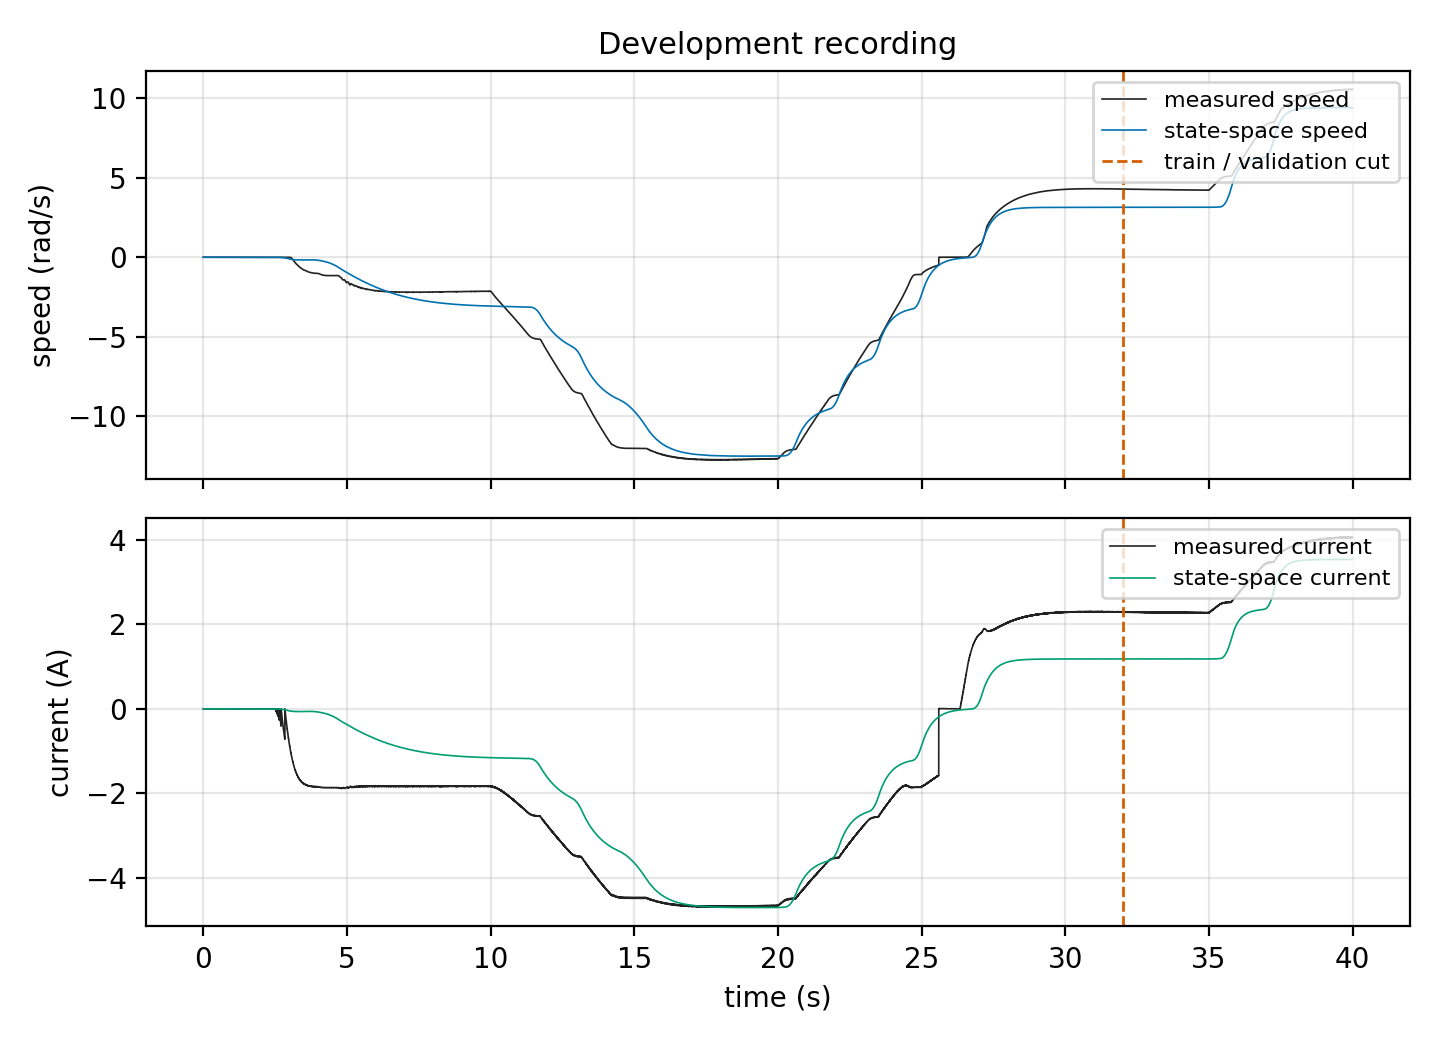
\includegraphics[width=0.92\textwidth]{../results/figures/eda_development.png}
\caption{Development recording after alignment to 1~ms. The dashed line is the training cut at 32~s.}
\label{fig:eda}
\end{figure*}

\subsection{Split, scaling, and leakage}
Training uses every development row with $t < 32$~s (32{,}000 rows). Validation uses the other 8{,}001 rows. The cut falls on a plateau near $4.3$~rad/s, not in the middle of a large transient. The test run is never used to choose a degree, a width, a learning rate, or a seed.

Each of the three inputs is standardized with the training mean and standard deviation. Validation and test rows use that same transform. The target is left in radians per second, so the reported errors are physical. Rows are not shuffled across the cut. Stochastic gradient descent shuffles only the training rows, and it does so independently in each epoch.

\section{Methods}
\subsection{Baseline and polynomial models}
The baseline predicts $\hat{\omega}(t) = \omega_{\mathrm{model}}(t)$. It has no fitted weights.

The learned polynomials use every monomial in the three standardized inputs of total degree $0$ through $d$, for $d \in \{2,3,4,5\}$. That is 10, 20, 35, and 56 terms, including the constant. No ridge term is added. Ordinary least squares solves $\min_{w} \|\Phi w - \omega\|_{2}$ with a rank-revealing solver. Stochastic gradient descent minimizes the mean squared error
\begin{equation}
L(w) = \frac{1}{B}\sum_{i \in \mathcal{B}} (\phi_{i}^{\top} w - \omega_{i})^{2}
\end{equation}
with the gradient $(2/B)\Phi_{\mathcal{B}}^{\top}(\Phi_{\mathcal{B}} w - \omega_{\mathcal{B}})$. The constant weight starts at zero. The other weights are drawn from the He normal, with variance $2/(p-1)$ for $p$ columns. The learning rates are $10^{-3}$, $10^{-2}$, and $10^{-1}$. Each run uses 100 epochs and minibatches of 256. The selection seed is 525.

\subsection{Neural network}
The second model class is a network with one hidden layer of 16 or 32 ReLU units and a linear output. Its input is the same three standardized values, not the polynomial expansion. Hidden weights use the He scale $\sqrt{2/3}$, output weights use $\sqrt{2/H}$, and both biases start at zero. Training minimizes the same mean squared error with plain minibatch gradient descent, the same three learning rates, the same batch size, and the same 100 epochs. There is no momentum and no early stopping. The epoch budget is part of the method, not a result that is tuned after the fact.

\subsection{Selection and uncertainty}
Every configuration is scored by validation RMSE. Divergent runs, those that produce a non-finite weight, are discarded. Ties would be broken toward the simpler setting. The winning least-squares degree, the winning gradient setting, and the winning network are kept. Least squares is deterministic, so it is solved once and applied to the test run. The winning gradient setting and the winning network are retrained from seeds 525 through 529, and the test RMSE is summarized by the sample mean and standard deviation. The test labels are read only after this selection.

\section{Results}
Table~\ref{tab:val} lists every finite configuration. Ordinary least squares lowers the training RMSE as the degree grows, from 0.538 at degree 2 to 0.123 at degree 5, while the validation RMSE rises from 1.45 to 138. The condition number of the singular values grows from $1.41 \times 10^{6}$ at degree 2 to $3.91 \times 10^{15}$ at degree 5, so the high-degree normal equations are numerically unstable even though the raw inputs were standardized. Learning rate $0.1$ diverges for every polynomial and for the 32-unit network. The selected models are degree-2 least squares, degree-3 gradient descent at learning rate $10^{-3}$ (validation RMSE 0.387), and the 32-unit network at learning rate $10^{-2}$ (validation RMSE 0.713). The state-space baseline sits at validation RMSE 1.113. The gradient model is the overall validation winner.

\begin{table}[!t]
\caption{Validation RMSE on the last 8~s of the development run. Training RMSE is shown for the least-squares degree sweep.}
\label{tab:val}
\centering
\footnotesize
\begin{tabular}{lcc}
\toprule
Configuration & Val.\ RMSE & Train RMSE \\
\midrule
State-space speed & 1.113 & 1.040 \\
Least squares, degree 2 & 1.452 & 0.538 \\
Least squares, degree 3 & 3.147 & 0.265 \\
Least squares, degree 4 & 3.045 & 0.180 \\
Least squares, degree 5 & 137.7 & 0.123 \\
SGD, degree 2, $10^{-3}$ & 0.953 & 0.615 \\
SGD, degree 2, $10^{-2}$ & 0.975 & 0.607 \\
SGD, degree 3, $10^{-3}$ & \textbf{0.387} & 0.479 \\
SGD, degree 3, $10^{-2}$ & 2.696 & 0.431 \\
SGD, degree 4, $10^{-3}$ & 14.27 & 0.503 \\
SGD, degree 5, $10^{-3}$ & 37.27 & 0.473 \\
Network, 16 units, $10^{-3}$ & 1.016 & 0.326 \\
Network, 16 units, $10^{-2}$ & 1.491 & 0.204 \\
Network, 16 units, $10^{-1}$ & 3.397 & 2.172 \\
Network, 32 units, $10^{-3}$ & 0.807 & 0.328 \\
Network, 32 units, $10^{-2}$ & 0.713 & 0.212 \\
\bottomrule
\end{tabular}
\end{table}

Figure~\ref{fig:curves} shows why a fixed epoch budget matters. For the selected gradient model, validation error falls, rebounds, and returns to its lowest region only near epoch 100. For the selected network, validation error is lowest near epoch 20 and then settles near 0.71 while the training error keeps falling. Stopping at the validation minimum would have been a different method. This study reports the 100-epoch weights.

\begin{figure*}[!t]
\centering
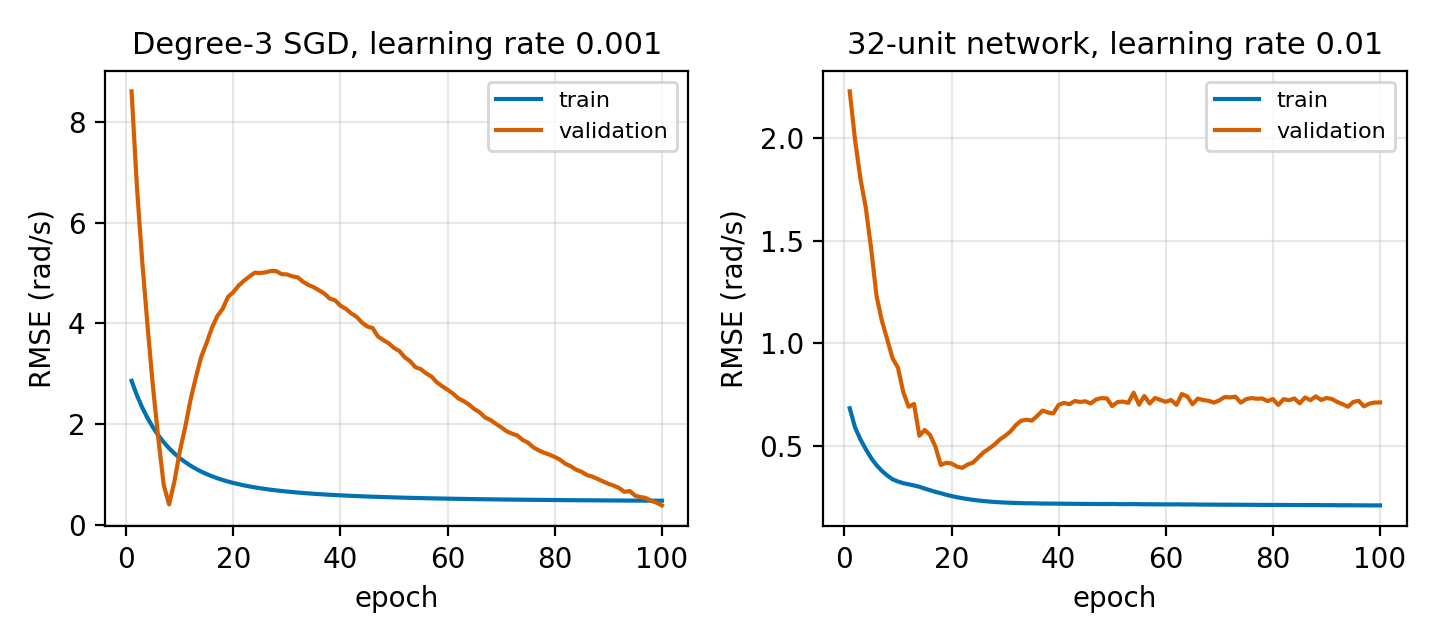
\includegraphics[width=0.92\textwidth]{../results/figures/learning_curves.png}
\caption{Training and validation RMSE for the two selected stochastic models. Both curves use seed 525.}
\label{fig:curves}
\end{figure*}

On the locked test run the baseline RMSE is 0.890 (MSE 0.792, MAE 0.704). Degree-2 least squares is worse, at RMSE 1.061. The degree-3 gradient model, over five seeds, has test RMSE $0.768 \pm 0.043$, mean MSE 0.592, and mean MAE 0.575. The seed used for selection scores 0.744. The 32-unit network scores $1.210 \pm 0.154$ and does not beat the baseline. The five gradient seeds score 0.744, 0.817, 0.749, 0.721, and 0.810. The five network seeds score 1.093, 1.316, 1.353, 1.001, and 1.287.

On the selected cubic model the largest weights, in the standardized coordinates, are the bias ($-3.37$), measured current ($+2.29$), model current ($+1.83$), measured-current squared ($-1.26$), and model speed ($+1.22$). The fit is not a small correction sitting on top of $\omega_{\mathrm{model}}$. Model speed is only the fifth-largest weight, and the current terms, including the $i_{a} i_{\mathrm{model}}$ interaction ($-0.77$), carry more of the estimate. Table~\ref{tab:time} splits the seed-525 gradient prediction into 10~s blocks. The average gain is not uniform: the model is worse than the state-space speed on the first 10~s and better after 20~s, especially on the final plateau.

\begin{table}[!t]
\caption{Test RMSE by time block for the state-space baseline and for the degree-3 SGD model at seed 525.}
\label{tab:time}
\centering
\begin{tabular}{lcc}
\toprule
Interval & Baseline & Degree-3 SGD \\
\midrule
0--10~s & 0.641 & 0.978 \\
10--20~s & 1.024 & 0.941 \\
20--30~s & 1.165 & 0.592 \\
30--40~s & 0.592 & 0.155 \\
\midrule
Full test & 0.890 & 0.744 \\
\bottomrule
\end{tabular}
\end{table}

Figure~\ref{fig:trace} overlays the three speeds. The lower panel zooms to 25~s through 35~s. On that window the degree-3 model has RMSE 0.310, against 1.142 for the state-space speed. The physics trace sits below the measurement until 30~s and then overshoots the plateau, while the cubic model stays closer throughout. Figure~\ref{fig:residual} shows the same error as a time series: a positive bias through much of the first half, a sharp negative spike near 22~s, and a small residual on the final plateau.

\begin{figure*}[!t]
\centering
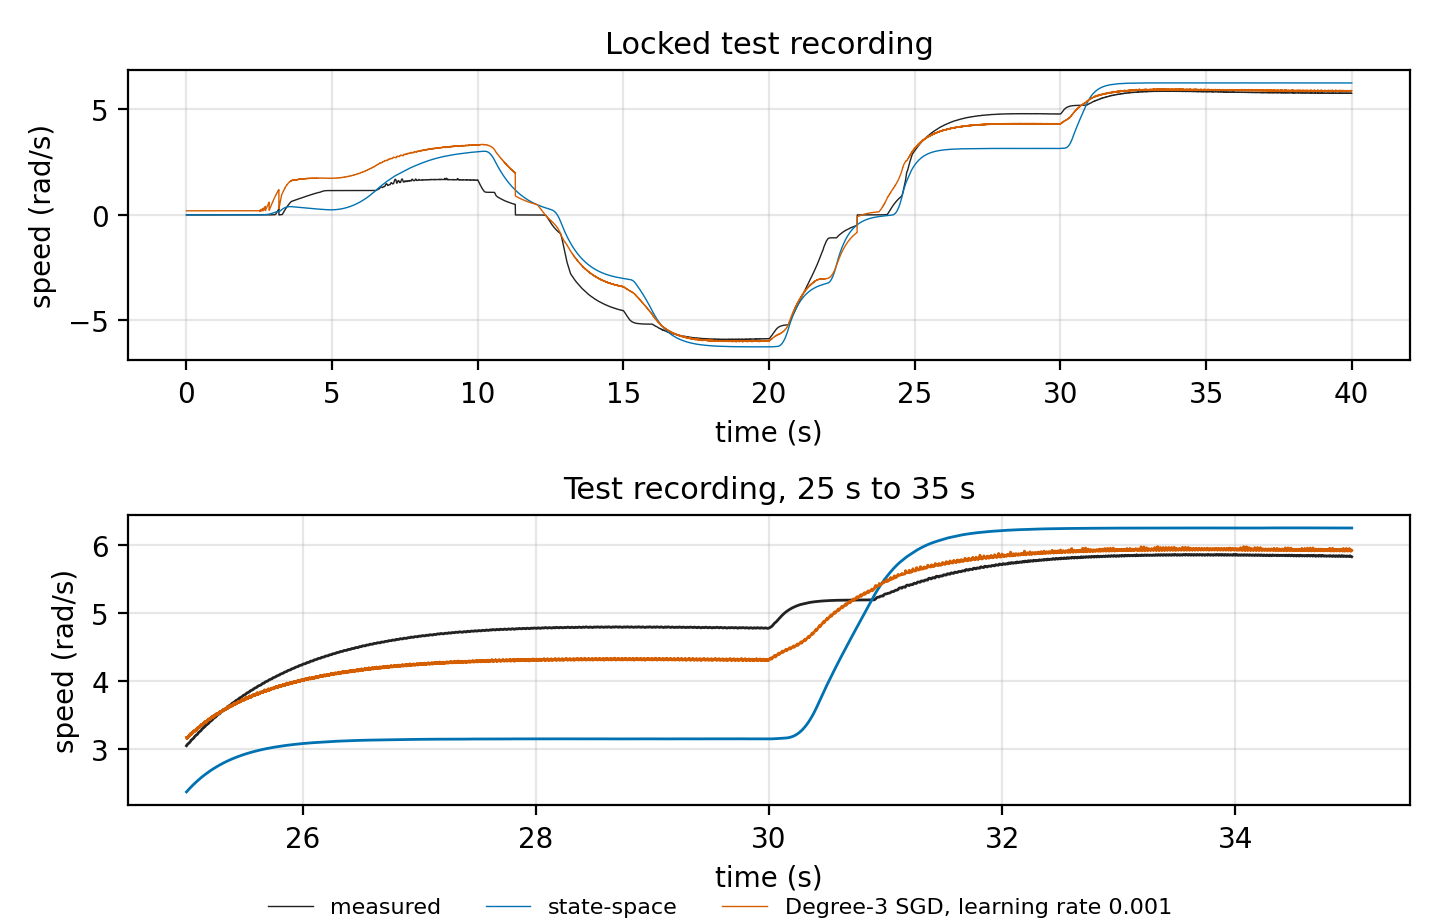
\includegraphics[width=0.92\textwidth]{../results/figures/test_trace.png}
\caption{Locked test recording. The lower panel is 25~s to 35~s. The orange trace is the degree-3 SGD model trained with seed 525.}
\label{fig:trace}
\end{figure*}

\begin{figure*}[!t]
\centering
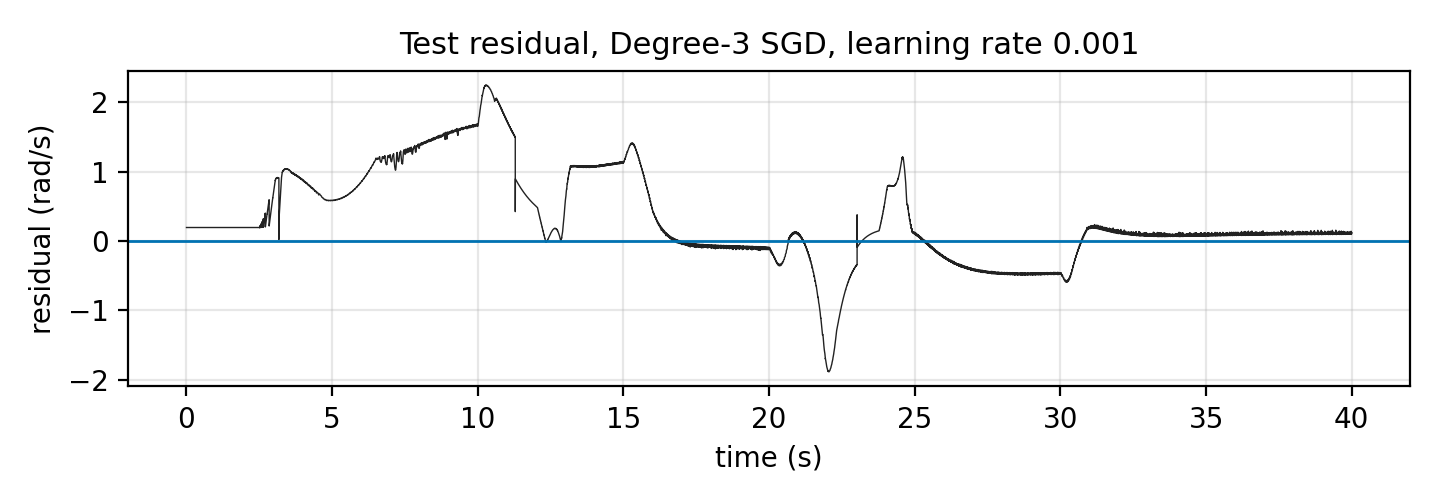
\includegraphics[width=0.78\textwidth]{../results/figures/test_residual.png}
\caption{Test residual of the seed-525 degree-3 SGD model. Positive values are over-predicted speed.}
\label{fig:residual}
\end{figure*}

The five seeds are not interchangeable. Table~\ref{tab:seeds} shows the spread. The cubic model stays inside a band of about $0.10$~rad/s. The network moves by about $0.35$~rad/s. A single training run would have been a misleading summary of the network and an acceptable summary of the cubic model.

\begin{table}[!t]
\caption{Test RMSE (rad/s) at each uncertainty seed. Seed 525 is the seed used to choose the hyperparameters.}
\label{tab:seeds}
\centering
\begin{tabular}{lcc}
\toprule
Seed & Degree-3 SGD & 32-unit network \\
\midrule
525 & 0.744 & 1.093 \\
526 & 0.817 & 1.316 \\
527 & 0.749 & 1.353 \\
528 & 0.721 & 1.001 \\
529 & 0.810 & 1.287 \\
\bottomrule
\end{tabular}
\end{table}

\section{Discussion}
The degree sweep is an ablation of one model class. Training error alone would have selected degree 5. Validation error selects degree 3 and a small step size, and that choice is the only polynomial setting that beats the baseline on the test run. The gap between least squares and gradient descent at the same degree is a numerical result, not evidence that the cubic polynomial is a different function class. With a condition number past $10^{6}$, the least-squares coefficients are not a trustworthy evaluation of that polynomial. A small step size, stopped at 100 epochs, never forms those unstable coefficients.

The network is the more flexible of the two learned models and the one with the lower training error. It loses on the test run. Two facts in the study point the same way. The validation curve rises after epoch 20, so the agreed horizon keeps weights that validation had already started to reject. The test motion is also smaller than the development motion, and a flexible fit of the larger swings need not transfer. Five seeds move the network's test RMSE by about $0.15$~rad/s, several times the spread of the cubic gradient model.

The residual is structured. An encoder replacement that is accurate on average and biased by 1~rad/s on a plateau would still pull a speed controller. The first 10~s are the concrete counterexample: overall RMSE improved, and that block got worse. The 25--35~s window is the other side of the same fact. A later controller study would have to score peak error and time-in-band, not only RMSE.

The implementation is NumPy 2.2.3 and Matplotlib 3.10.1 on Python 3.13. \texttt{python test\_sensorless.py} checks the polynomial basis, the training-only scaler, and that both optimizers reduce error on a known target. \texttt{python run\_experiments.py} refits every configuration from seed 525 and writes \texttt{results/summary.json}.

The recordings are simulated. They do not include brush friction drift, a passenger's weight, or a wheel leaving the ground. The current and speed units are an assumption taken from the scale of the traces. No armature voltage or speed command was stored in the files, so the estimator cannot be asked to use them. Putting this estimate inside the wheelchair loop, without a hardware trial and a bound on the residual, would be an unsafe use of a class project. The ethical point is narrow and practical. The rider cannot correct a bad speed loop with their hands, so a simulation RMSE is not a deployment argument.

Two changes would be a different study, and they are named here so they are not smuggled into this one. Early stopping at the validation minimum would keep an earlier network and might change the test ranking. It was not used. Scaling each polynomial column, instead of only the three raw inputs, would lower the condition number of the least-squares problem. It was not used, because the agreed expansion is the monomial basis of the standardized inputs. Either change could make least squares look more competitive. The numbers above are for the method that was actually run.

A speed loop also needs a bound, not only a mean square. The 0--10~s block is the bound this recording supports: the selected model can be worse than the physics trace by several tenths of a radian per second for ten seconds at a time. That block, not the full-run average, is the number to put next to a controller gain.

\section{Conclusion}
A cubic polynomial trained by stochastic gradient descent, with inputs standardized on the training slice and with the degree and the learning rate chosen on a later slice of the same run, estimates brushed-DC shaft speed more accurately than the state-space speed on a locked second recording: $0.768 \pm 0.043$~rad/s against $0.890$~rad/s. Ordinary least squares on the same polynomial family overfits as the degree rises, and a 32-unit ReLU network does not beat the baseline once the epoch budget and the test recording are honored. The remaining error is systematic in time. That is the quantity a wheelchair speed loop would feel.

\begin{thebibliography}{4}
\bibitem{kalman1960}
R.~E. Kalman, ``A new approach to linear filtering and prediction problems,'' \emph{J. Basic Eng.}, vol.~82, no.~1, pp.~35--45, 1960.
\bibitem{hastie2009}
T.~Hastie, R.~Tibshirani, and J.~Friedman, \emph{The Elements of Statistical Learning}, 2nd~ed. New York, NY, USA: Springer, 2009.
\bibitem{goodfellow2016}
I.~Goodfellow, Y.~Bengio, and A.~Courville, \emph{Deep Learning}. Cambridge, MA, USA: MIT Press, 2016.
\bibitem{he2015}
K.~He, X.~Zhang, S.~Ren, and J.~Sun, ``Delving deep into rectifiers: Surpassing human-level performance on ImageNet classification,'' in \emph{Proc. IEEE Int. Conf. Comput. Vis.}, 2015, pp.~1026--1034.
\end{thebibliography}

\clearpage
\onecolumn
\section*{Contribution Statement}
This page is outside the report page limit.

Mohammad Elmougey and Heinz Veintimilla shared the problem definition, the Simulink recordings, the experimental design, the implementation, this report, and the presentation.

\end{document}
